\section{Исследовательский раздел}
\subsection{Условия исследований}
Исследование проводилось на персональном вычислительной машине со следующими характеристиками:

\begin{itemize}
\item процессор Apple M1 Pro,
\item операционная система Ventura 13.5.2,
\item 32 Гб оперативной памяти.
\end{itemize}

Оценки RMSE и MAE определялись внутренними средствами библиотеки scikit-surprise.

Так как рекомендации, полученные с использование TF-IDF носят дополнительный характер, их вес составляет $0.2$, в то время как вес рекомендаций SVD составляет $0.8$.

\subsection{Зависимость значения метрики RMSE алгоритмов}

На рисунке \ref{img:1} представлен график зависимости значения метрики RMSE от значения параметра регуляризации.

\begin{figure}[H]
	\centering
	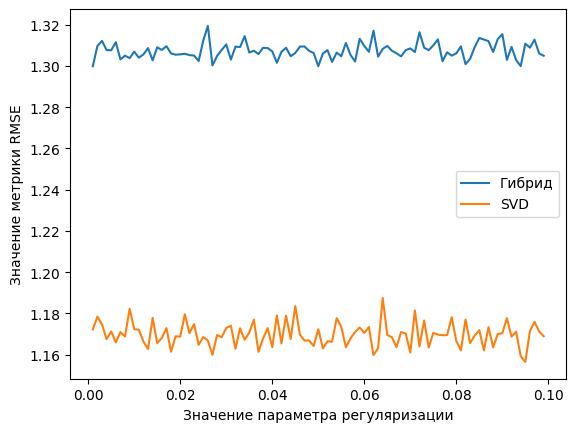
\includegraphics[width=\textwidth]{inc/1.png}
	\caption{ График зависимости значения метрики RMSE от значения параметра регуляризации.}
	\label{img:1}
\end{figure}

На рисунке \ref{img:2} представлен график зависимости значения метрики RMSE от значения параметра количества эпох.

\begin{figure}[H]
	\centering
	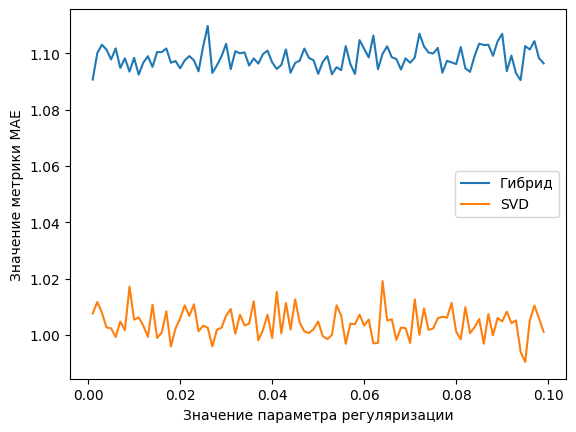
\includegraphics[width=\textwidth]{inc/2.png}
	\caption{ График зависимости значения метрики RMSE от значения параметра количества эпох.}
	\label{img:2}
\end{figure}

\subsection{Зависимость значения метрики MAE алгоритмов}

На рисунке \ref{img:3} представлен график зависимости значения метрики MAE от значения параметра регуляризации.

\begin{figure}[H]
	\centering
	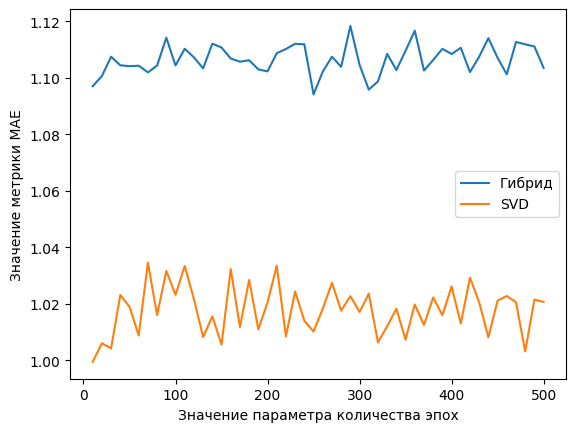
\includegraphics[width=\textwidth]{inc/3.png}
	\caption{ График зависимости значения метрики MAE от значения параметра регуляризации.}
	\label{img:3}
\end{figure}

На рисунке \ref{img:4} представлен график зависимости значения метрики RMSE от значения параметра количества эпох.

\begin{figure}[H]
	\centering
	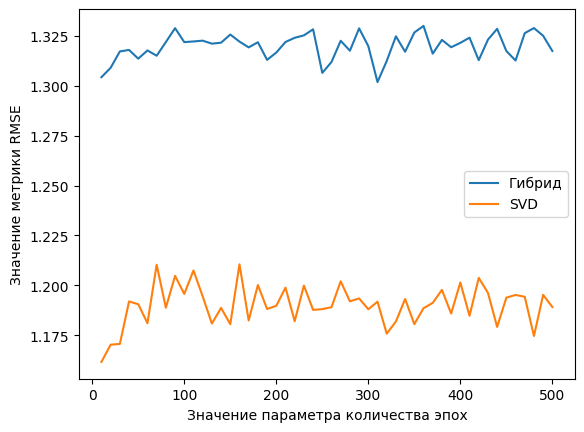
\includegraphics[width=\textwidth]{inc/4.png}
	\caption{ График зависимости значения метрики MAE от значения параметра количества эпох.}
	\label{img:4}
\end{figure}


\subsection*{Заключение}

В результате проведенных исследований легко увидеть, что реализованная гибридная система уступает обычному алгоритму SVD, причем разница и по MAE, и по RMSE составляет в среднем 10 процентов. Таким образом, можно сделать вывод, что либо были подобраны неправильные веса систем, либо слишком мала выборка дополнительных рекомендаций, вносимых с использованием TF-IDF.

Так или иначе, сама реализация гибридной системы не столько удовлетворяет потребности увеличения точности, сколько большему разнообразию рекомендаций.